\documentclass[xcolor=table]{beamer}
\mode<presentation>
\usetheme{CambridgeUS}
\usepackage[english, russian]{babel}
\usepackage[utf8]{inputenc}
\usepackage[T2A]{fontenc}
\usepackage{sansmathaccent}
\usepackage{alltt}
\usepackage[table]{xcolor}
\linespread{0.8}
\usepackage{minted}
%\usepackage{setspace}

\pdfmapfile{+sansmathaccent.map}
\title[Software Design]{Тестирование}
\author{Наумов Д.А., доц. каф. КТ}
\date[08.11.2020] {Основы программной инженерии, 2020}

\begin{document}

%ТИТУЛЬНЫЙ СЛАЙД
\begin{frame}
  \titlepage
\end{frame}
  
%СОДЕРЖАНИЕ ЛЕКЦИИ
\begin{frame}
  \frametitle{Содержание лекции}
  \tableofcontents  
\end{frame}

\section{Тестирование: понятия, процесс}

\begin{frame}
	\linespread{1.0}
	\begin{block}{Тестирование (software testing)}
		деятельность, выполняемая для оценки и улучшения качества программного обеспечения. Эта деятельность, в общем случае, базируется на обнаружении \textit{дефектов} и \textit{проблем} в программных системах.
	\end{block}

	Тестирование программных систем состоит из:
	\begin{itemize}
		\item динамической верификации поведения программ 
		\item на конечном (ограниченном) наборе тестов (set of test cases)
		\item выбранных соответствующим образом из обычно выполняемых действий прикладной области
		\item и обеспечивающих проверку соответствия ожидаемому поведению системы.
	\end{itemize}
	Сегодня тестирование рассматривается как деятельность, которую необходимо проводить \textbf{на протяжении всего процесса разработки и сопровождения} и является важной частью конструирования программных продуктов.
\end{frame}

\begin{frame}
	\linespread{0.8}
	\begin{block}{Динамичность (dynamic)}
		предполагает выполнение тестируемой программы с заданными входными данными.
	\end{block}
	\begin{block}{Конечность (ограниченность, finite)}
		предполагает компромисс между ограниченными ресурсами и заданными сроками, с одной стороны, и практически неограниченными требованиями по тестированию, с другой.
	\end{block}
	\begin{block}{Выбор (selection) сценариев тестирования}
		 на основе техники анализа рисков, анализа требований и экспертизе в области тестирования и заданной прикладной области.
	\end{block}
	\begin{block}{Ожидаемое поведение (expected behaviour)}
		может рассматриваться в контексте:
		\begin{itemize}
			\item пользовательских ожиданий (testing for validation)
			\item спецификации (testing for verification) 
			\item на основе неявных требований или обоснованных ожиданий.
		\end{itemize}		 
	\end{block}			
\end{frame}

\begin{frame}
	\linespread{1.0}
	\begin{itemize}
		\item Важно четко разделять \textbf{причину нарушения работы} прикладных систем, обычно описываемую терминами \textbf{недостаток} или \textbf{дефект}, и наблюдаемый нежелательный эффект, вызываемый этими причинами – \textbf{сбой}. 
		\item Термин ошибка, в зависимости от контекста, может описывать и как \textbf{причину сбоя}, и сам \textbf{сбой}. 
		\item Тестирование позволяет обнаружить дефекты, приводящие к сбоям.
	\end{itemize}		 
	Необходимо понимать, что причина сбоя \textbf{не всегда может быть однозначно определена}. 

	\medskip	
	
	Не существует теоретических критериев, позволяющих гарантированно определить какой именно дефект приводит к наблюдаемому сбою	
\end{frame}

\begin{frame}{Модульное тестирование (Unit testing)}
	позволяет проверить функционирование отдельно взятого элемента системы. Что считать элементом – модулем системы определяется контекстом.
	\begin{figure}[h]
		\centering
		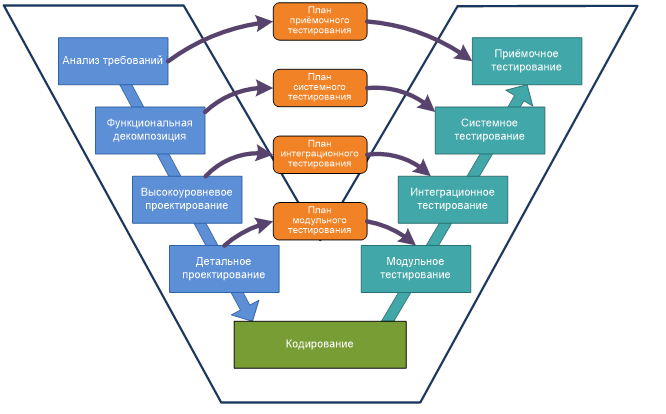
\includegraphics[scale=0.6]{images/testing-levels.png}
	\end{figure}
\end{frame}

\begin{frame}{Интеграционное тестирование (Integration testing)}
	является процессом проверки взаимодействия между программными компонентами/модулями. 
	\begin{figure}[h]
		\centering
		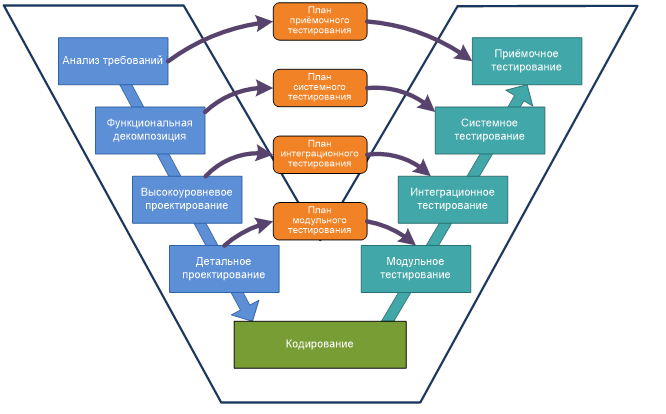
\includegraphics[scale=0.6]{images/testing-levels.png}
	\end{figure}
\end{frame}

\begin{frame}{Системное тестирование (System testing)}
	охватывает целиком всю систему и фокусируется на нефункциональных требованиях -– безопасности, производительности, точности, надежности т.п.  
	\begin{figure}[h]
		\centering
		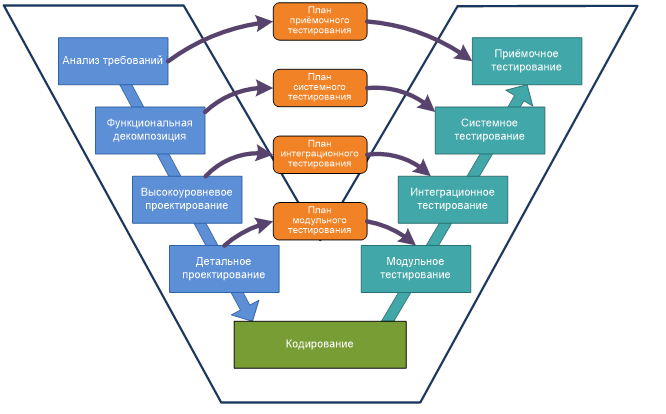
\includegraphics[scale=0.6]{images/testing-levels.png}
	\end{figure}
\end{frame}

\begin{frame}{Приёмочное тестирование (Acceptance/qualification testing)}
	Проверяет поведение системы на предмет удовлетворения требований заказчика. 
	\begin{figure}[h]
		\centering
		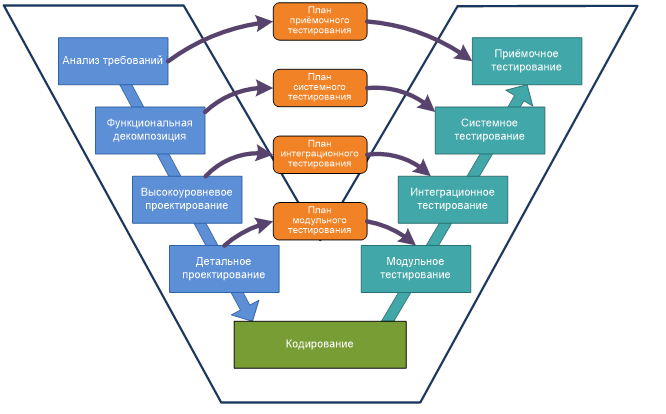
\includegraphics[scale=0.6]{images/testing-levels.png}
	\end{figure}
\end{frame}

\begin{frame}{Цели тестирования}
	\begin{itemize}
		\item \textbf{Установочное тестирование} (Installation testing) -- проверка процедуры инсталляции системы в целевом окружении.
		\item \textbf{Альфа- и бета-тестирование} (Alpha and beta testing) -- перед массовым использованием необходдимо пройти стадии альфа (внутреннее пробное использование) и бета (пробное использование с привлечением отобранных внешних пользователей) версий.
		\item \textbf{Функциональные тесты}/тесты соответствия 
(Conformance testing/Functional testing/Correctness testing) -- проверка соответствия системы, предъявляемым к ней требованиям, описанным на уровне спецификации поведенческих характеристик.
		\item \textbf{Достижение и оценка надежности} (Reliability achievement and evaluation)
		\item \textbf{Регрессионное тестирование} (Regression testing) -- повторное выборочное тестирование системы или компонент для проверки сделанных модификаций.
	\end{itemize}		 
\end{frame}

\begin{frame}{Цели тестирования}
	\begin{itemize}
		\item \textbf{Тестирование производительности} (Performance testing) --
проверка удовлетворения специфических требований, предъявляемых к параметрам производительности.	
		\item \textbf{Нагрузочное тестирование} (Stress testing) -- выполнение программной системы c повышением нагрузки.
		\item \textbf{Сравнительное тестирование} (Back-to-back testing) -- сравнение двух версий системы.		
		\item \textbf{Восстановительные тесты} (Recovery testing) -- проверка возможностей рестарта системы в случае непредусмотренной катастрофы (disaster).		
		\item \textbf{Конфигурационное тестирование} (Configuration testing) -- проверка поведения и работоспособности системы в различных конфигурациях.
		\item\textbf{Тестирование удобства} и простоты использования (Usability testing) -- проверка, насколько легко конечный пользователь системы может ее освоить.
	\end{itemize}		 
\end{frame}

\begin{frame}{Техники тестирования}
	\begin{enumerate}
		\item Техники, базирующиеся на интуиции и опыте инженера 
		\begin{itemize}
			\item Специализированное тестирование
			\item Исследовательское тестирование
		\end{itemize}
		\item Техники, базирующиеся на спецификации
		\begin{itemize}
			\item Эквивалентное разделение приложения
			\item Анализ граничных значений
			\item Таблицы принятия решений
			\item Тесты на основе конечного автомата
			\item Тестирование на основе формальной спецификации
			\item Случайное тестирование
		\end{itemize}		
		\item Техники, ориентированные на код
		\begin{itemize}
			\item Тесты, базирующиеся на блок-схеме 
			\item Тесты на основе потоков данных 
		\end{itemize}		
		\item Тестирование, ориентированное на дефекты 
		\begin{itemize}
			\item Предположение ошибок 
			\item Тестирование мутаций 
		\end{itemize}				
		\item Техники, базирующиеся на условиях использования
		\begin{itemize}
			\item Операционный профиль
			\item Тестирование, базирующееся на надежности инженерного процесса
		\end{itemize}	
	\end{enumerate}
\end{frame}

\begin{frame}{Процесс и документирование}
	Работы по тестированию должны быть организованы в единый процесс, на основе учета четырех элементов и связанных с ними факторов: 
	\begin{enumerate}
		\item людей (в том числе, в контексте организационной структуры и культуры),
		\item инструментов, 
		\item регламентов,
		\item количественных оценок (измерений). 
	\end{enumerate}
	
	\textbf{Документация} -- составная часть формализации процесса тестирования. 	Стандарт IEEE 829-98 <<Standard for Software Test Documentation>>, предоставляющий описание тестовых документов, их связей между собой и с процессом тестирования:
	\begin{itemize}
		\item план тестирования;
		\item спецификация процедуры тестирования;
		\item спецификация тестов;
		\item лог тестов;
		\item и др.	
	\end{itemize}	
\end{frame}

\section{Тестирование в Python: doctest}

\begin{frame}
  \frametitle{Содержание лекции}
  \tableofcontents[current]
\end{frame}

\begin{frame}
	\linespread{1.0}
	\begin{block}{REPL (read-eval-print loop -- цикл <<чтение-вычисление-вывод>>)}
		форма организации простой интерактивной среды программирования в рамках средств интерфейса командной строки.	
	\end{block}

	Пользователь может вводить выражения, которые среда тут же будет вычислять, а результат вычисления отображать пользователю. 
	\begin{itemize}
		\item функция \textit{read} читает одно выражение и преобразует его в соответствующую структуру данных в памяти;
		\item функция \textit{eval} принимает одну такую структуру данных и вычисляет соответствующее ей выражение;
		\item функция \textit{print} принимает результат вычисления выражения и печатает его пользователю.
	\end{itemize}
\end{frame}

\begin{frame}[t, fragile]{Doctest}
	\linespread{1.0}
	\begin{block}{Модуль Doctest}
		ищет фрагменты текста, которые выглядят как интерактивные \textit{python}- сессии. Далее выполняет сеансы и проверяет, совпадает ли с тем что указано в docstring.
	\end{block}
	\begin{itemize}
		\item использование \textit{doctest} выглядит, как будто пишем код в \textit{REPL}.
		\item можно применять для тестирования как функций, так и классов;
	\end{itemize}
	
	\medskip
	
	Напишем тесты для функции \textit{moo}:
	\begin{minted}{python}
def moo(oos=2, end=""):
    '''Издать мычание длиной oos с end в конце'''
    return "M"+"o"*oos+end	
	\end{minted}
\end{frame}

\begin{frame}[t, fragile]{Ручное тестирование}	
	\begin{minted}{python}
> python -i Moo.py

>>> moo()
'Moo'
>>> moo(4)
'Moooo'
>>> moo(0)
'M'
>>> moo(end='!')
'Moo!'
>>> moo(0,'?')
'M?'
	\end{minted}
\end{frame}

\begin{frame}[t, fragile]
	\begin{minted}{python}
def moo(oos=2, end=""):
''' Издать мычание длиной oos с end в конце
    Оба параметра необязательны:
>>> moo()
'Moo'
    Первый задаёт количество букв 'o' в слове 'Moo'
>>> moo(4)
'Mooooo'
    Букв 'o' может и не быть
>>> moo(0)
'M'
    Второй задаёт символ после всех 'o' (по умолчанию — ничего)
>>> moo(end='!')
'Moo!'
>>> moo(0,'?')
'M?'
    '''
    return "M"+"o"*oos+end
	\end{minted}
\end{frame}

\begin{frame}[t, fragile]{Тестирование}
	\begin{minted}{python}
> python -m doctest Moo.py

*******************************************************
File "Moo.py", line 13, in Moo.moo
Failed example:
    moo(4)
Expected:
    'Mooooo'
Got:
    'Moooo'
*******************************************************
1 items had failures:
   1 of   5 in Moo.moo
***Test Failed*** 1 failures.
	\end{minted}
\end{frame}

\begin{frame}[t, fragile]{Отчет с успешными тестами}
	\begin{minted}{python}
> python3 -m doctest -v Moo.py

Trying:
    moo()
Expecting:
    'Moo'
ok
Trying:
    moo(4)
Expecting:
    'Mooooo'
********************************************************
File "Moo.py", line 13, in Moo.moo
Failed example:
    moo(4)
Expected:
    'Mooooo'
Got:
    'Moooo'
	\end{minted}    
\end{frame}

\begin{frame}[t, fragile]{Отчет с успешными тестами}
	\begin{minted}{python}
Trying:
    moo(0)
Expecting:
    'M'
ok
Trying:
    moo(end='!')
Expecting:
    'Moo!'
ok
Trying:
    moo(0,'?')
Expecting:
    'M?'
ok
	\end{minted}    
\end{frame}

\begin{frame}[t, fragile]{Отчет с успешными тестами}
	\begin{minted}{python}
1 items had no tests:
    Moo	
*********************************************************
1 items had failures:
   1 of   5 in Moo.moo
5 tests in 2 items.
4 passed and 1 failed.
***Test Failed*** 1 failures.
	\end{minted}
\end{frame}

\begin{frame}[t, fragile]{Тестирование исключений}
	\begin{minted}{python}
> python -i Moo

>>> moo("QQ")

Traceback (most recent call last):
  File "<stdin>", line 1, in <module>
  File "Moo.py", line 33, in moo
    return "M"+"o"*moos+end
TypeError: can't multiply sequence by non-int of type 'str'

>>>
	\end{minted}
\end{frame}

\begin{frame}[t, fragile]{Тестирование исключений}
	Важны только три строчки, остальные можно не включать в \textit{docstring}:
	\begin{minted}{python}
def moo(oos=2, end=""):
    ''' Издать мычание длиной oos с end в конце
		...
		Здесь должно быть исключение:
		
>>> moo("QQ")
Traceback (most recent call last):
TypeError: can't multiply sequence by non-int of type 'str'
	'''
	\end{minted}
\end{frame}

\begin{frame}[t, fragile]{Перенос тестов во внешний файл}
	\begin{block}{Файл exttest.rst (.rst -- для Sphinx)}
		\begin{minted}{python}
External test
=============

Using Moo
---------

Start from importing 'Moo' module:

        >>> import Moo

Then call 'moo':
        >>> Moo.moo(5)
        'Mooooo'	
    	\end{minted}
	\end{block}
	\begin{block}{Файл exttest.py}
		\begin{minted}{python}
import doctest
doctest.testfile("exttest.rst")	
		\end{minted}
	\end{block}
\end{frame}

\begin{frame}[t, fragile]{Файл для запуска тестов}
	\begin{minted}{python}
> python exttest.py -v

Trying:
    import Moo
Expecting nothing
ok
Trying:
    Moo.moo(5)
Expecting:
    'Mooooo'
ok
1 items passed all tests:
   2 tests in exttest.rst
2 tests in 1 items.
2 passed and 0 failed.
Test passed.	
	\end{minted}
\end{frame}

\begin{frame}[t, fragile]{Тестирование классов}
	\begin{minted}{python}
class Test(object):
    """
    >>> a=Test(5)
    >>> a.multiply_by_2()
    10
    """
    def __init__(self, number):
        self.number = number

    def multiply_by_2(self):
        return self.number*2

if __name__ == "__main__":
    import doctest
    doctest.testmod()        
	\end{minted}
\end{frame}

\begin{frame}[t, fragile]{Тестирование классов}
	\begin{minted}{python}
> python example.py -v  
     
Trying:
    a=Test(5)
Expecting nothing
ok
Trying:
    a.multiply_by_2()
Expecting:
    10
ok
3 items had no tests:
    __main__
    __main__.Test.__init__
    __main__.Test.multiply_by_2
1 items passed all tests:
   2 tests in __main__.Test
2 tests in 4 items.
2 passed and 0 failed.
Test passed.       
	\end{minted}
\end{frame}

\section{Тестирование в Python: unittest}

\begin{frame}
  \frametitle{Содержание лекции}
  \tableofcontents[current]
\end{frame}

\begin{frame}[t, fragile]{Модульное тестирование при помощи unittest}
	Возможности \textit{unittest}:
	\begin{itemize}
		\item обнаружение и автоматическое исполнение тестов;
		\item настройка теста и его завершение;
		\item группирование тестов;
		\item статистика тестирования.
	\end{itemize}
	Чтобы создать тестовый случай, нужно:
	\begin{enumerate}
		\item создать класс, отнаследованный от \textit{unittest.TestCase};
		\item внутри этого класса добавить несколько методов, начинающихся со слова \textit{test}.
		\item каждый из этих методов должен тестировать какой-то из аспектов кода.
	\end{enumerate}
\end{frame}

\begin{frame}[t, fragile]{Тестирование свойств строк в Python}
	\begin{minted}{python}    
import unittest

class StringTestCase(unittest.TestCase):
    def test_sum(self):
        self.assertEqual("" + "", "")
        self.assertEqual("foo" + "bar", "foobar")

    def test_lower(self):
        self.assertEqual("FOO".lower(), "foo")
        self.assertTrue("foo".islower())
        self.assertFalse("Bar".islower())
       
if __name__ == '__main__':
    unittest.main()        
	\end{minted}
\end{frame}

\begin{frame}[t, fragile]{Unittest}
	Самые распространенные проверки:
	\begin{itemize}
		\item \textbf{self.assertEqual} – непосредственно проверяет, чтобы первый аргумент равнялся второму. Если это будет не так, то тест будет провален, и появится сообщение о том, что и где пошло не так.
		\item \textbf{self.assertTrue} – ожидает, что аргумент будет эквивалентен правде (True), а self.assertFalse – проверяет на ложь (False).	
	\end{itemize}
	
	~
	
	Запуск делается либо непосредственно из самой программы:
	\begin{minted}{python}    
if __name__ == '__main__':
    unittest.main()
	\end{minted}
	
	~
	
	А можно из консоли:
	\begin{minted}{python}    
> python -m unittest my_unittest.py
	\end{minted}
	
	~
	
	Модуль \textit{unittest} сам найдет все тестовые случаи и выполнит в них все тестовые функции.	
\end{frame}

\begin{frame}[t, fragile]{Unittest: Fixtures}
	\linespread{1.0}
	\textbf{Тестовые фикстуры} (test fixtures) –- особые условия, которые создаются для выполнения тестов:
	\begin{itemize}
		\item подготовка тестовых данных;
		\item создание подключений к БД, сервисам и т.п.
		\item создание заглушек (mock) для имитации компонентов программы;
		\item другие действия по поддержке рабочего окружения для проведения теста.	
	\end{itemize}
	Фикстуры могут быть созданы: 
	\begin{itemize}
		\item на уровне модуля с тестами; 
		\item на уровне отдельного класса (от unittest.TestCase); 
		\item для каждого метода в классе теста.
	\end{itemize}	
\end{frame}

\begin{frame}[t, fragile]{Unittest: Fixtures}
	\linespread{1.0}
	Фикстуры unittest:
	\begin{itemize}
		\item Метод \textbf{setUp()} вызывается перед каждым вызовом метода \textbf{test*} в классе тестового случая.
		\item Классовый метод \textbf{setUpClass()} вызывается один раз перед запуском тестов в классе тестового случая.
		\item Функция \textbf{setUpModule()} вызывается перед выполнением тестовых случаев в этом модуле.
	\end{itemize}		
	У них есть пары, предназначенные для освобождения ресурсов (закрытия соединений, удаления временных файлов и т.п.):
	\begin{itemize}
		\item \textbf{tearDown()} – после каждого метода-теста в классе.
		\item \textbf{tearDownClass()} – после всех тестов в классе.
		\item \textbf{tearDownModule()} – после всех классов в модуле.
	\end{itemize}		
\end{frame}

\begin{frame}[t, fragile]
	\linespread{0.8}
	\begin{minted}{python}
import unittest
class StringTestCase(unittest.TestCase):
    @classmethod
    def setUpClass(cls):
        print(' - set up class')
    def setUp(self):
        print(' - - set up method')
        self.foo = "foo"
        self.bar = "bar"
    def test_sum(self):
        self.assertEqual(self.foo + self.bar, "foobar")
    def test_lower(self):
        self.assertTrue(self.foo.islower())
    def tearDown(self):
        print(' - - tear down method')
    @classmethod
    def tearDownClass(cls):
        print(' - tear down class')
def setUpModule():
    print('set up module')
def tearDownModule():
    print('tear down module')
	\end{minted}
\end{frame}

\begin{frame}[t, fragile]
	\linespread{0.8}
	\begin{minted}{python}
...
if __name__ == '__main__':
    unittest.main()		
	\end{minted}
	
	\medskip
	
	Схема вызовов:
	\begin{minted}{bash}
set up module
 - set up class 
 - - set up method
 - - tear down method
 - - set up method
 - - tear down method
 - tear down class
tear down module
	\end{minted}
\end{frame}

\begin{frame}[t, fragile]{Пример}
	\linespread{0.8}
	\begin{minted}{python}
class MyTestCase(unittest.TestCase):
    @unittest.skip("всегда пропустить")
    def test_nothing(self):
        self.fail("не случится")
    @unittest.skipIf(mylib.__version__ < (1, 3),
        "эта версия библиотеки не поддерживается")
    def test_format(self):
        # этот тест работает только для определенных версий 
        pass
    @unittest.skipUnless(sys.platform.startswith("win"), 
        "надо Windows")
    def test_windows_support(self):
        # тест работает только на Windows
        pass
    def test_maybe_skipped(self):
        if not external_resource_available():
            self.skipTest("ресурс недоступен")
        # код дальше будет тестировать, если ресурс доступен
        pass
	\end{minted}
\end{frame}

\begin{frame}[t, fragile]{Пример пропуска класса}
	\linespread{1.0}
	\begin{minted}{python}
@unittest.skip("как пропустить класс")
class MySkippedTestCase(unittest.TestCase):
    def test_not_run(self):
        pass
	\end{minted}
	
	~
	
	Декоратор @unittest.expectedFailure говорит системе тестирования, что следующий метод 	должен провалиться (один из self.assert должен не сработать). 

	~	
	
	Таким образом, разработчик говорит, что он осведомлен, что данный тест пока проваливается, и в будущем к этому примут меры.
	\begin{minted}{python}
class ExpectedFailureTestCase(unittest.TestCase):
    @unittest.expectedFailure
    def test_fail(self):
        self.assertEqual(1, 0, "сломано")
	\end{minted}
\end{frame}

\begin{frame}[t, fragile]
	\linespread{0.8}
	Метод \textbf{self.assertRaises(SomeException)} проверяет, возбуждает ли код нужное исключение. 
	\begin{minted}{python}
import unittest

def my_div(a, b):
    return a // b
    
class MyDivTestCase(unittest.TestCase):
    def test_1(self):
        self.assertEqual(my_div(10, 2), 5)
        # при делении на 0 ждем исключение:
        with self.assertRaises(ZeroDivisionError):
            my_div(7, 0)
        # или так: исключение, функция, аргументы
        self.assertRaises(ZeroDivisionError, my_div, 5, 0)
        
unittest.main()
	\end{minted}
	Если из исключения нужно извлечь данные (к примеру, код ошибки):
	\begin{minted}{python}
with self.assertRaises(SomeException) as cm:
    do_something()
self.assertEqual(cm.exception.error_code, 3)
	\end{minted}
\end{frame}

\begin{frame}[t, fragile]
	\begin{figure}[h]
		\centering
		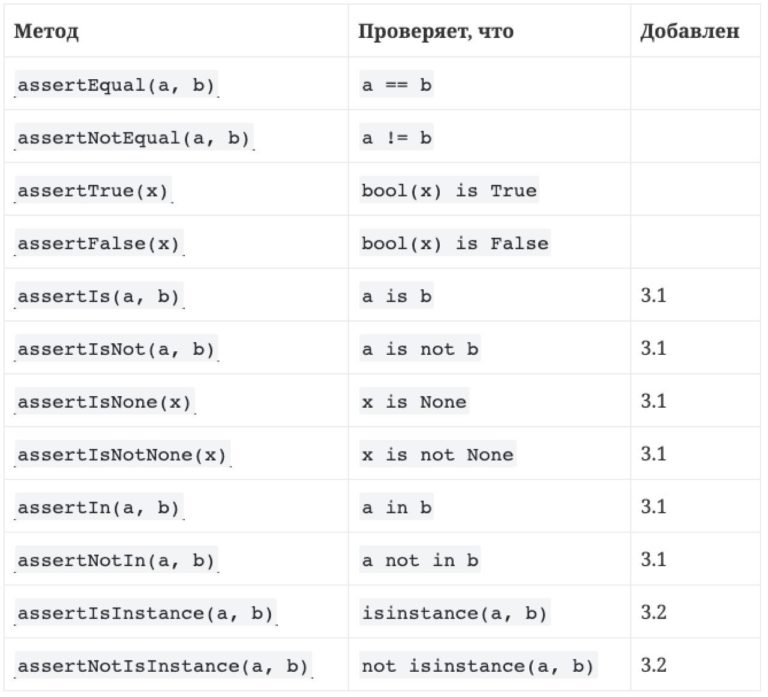
\includegraphics[scale=0.3]{images/unittest-checks.jpg}
	\end{figure}
\end{frame}

\section{Тестирование в Python: PyTest}

\begin{frame}
  \frametitle{Содержание лекции}
  \tableofcontents[current]
\end{frame}

\begin{frame}[t, fragile]{PyTest}
	\linespread{0.8}
	Библиотека \textit{PyTest} предоставляет более лаконичный и удобный инструментарий для написания тестов.

	~	
	Установка:
	\begin{minted}{bash}
	pip install pytest
	\end{minted}
	
	~
	
	Преимущества \textit{PyTest}:
	\begin{itemize}
		\item более краткий и красивый код;
		\item используется только один стандартный \textit{assert};
		\item возможность формирования подробного отчета;
		\item разнообразие фикстур;
		\item имеет плагин и интеграции с другими системами.
	\end{itemize}
	
	~
	
	В окружении, где установлен \textit{PyTest}, появится команда \textit{py.test}. Из терминала пишем:
	\begin{minted}{bash}
	py.test my_test_cases.py
	\end{minted}
\end{frame}

\begin{frame}[t, fragile]
	\begin{minted}{python}
import pytest

def setup_module(module):
    #init_something()
    pass
    
def teardown_module(module):
    #teardown_something()
    pass
    
def test_upper():
    assert 'foo'.upper() == 'FOO'
    
def test_isupper():
    assert 'FOO'.isupper()
    
def test_failed_upper():
    assert 'foo'.upper() == 'FOo'
	\end{minted}
\end{frame}

\begin{frame}[t, fragile]
	\begin{figure}[h]
		\centering
		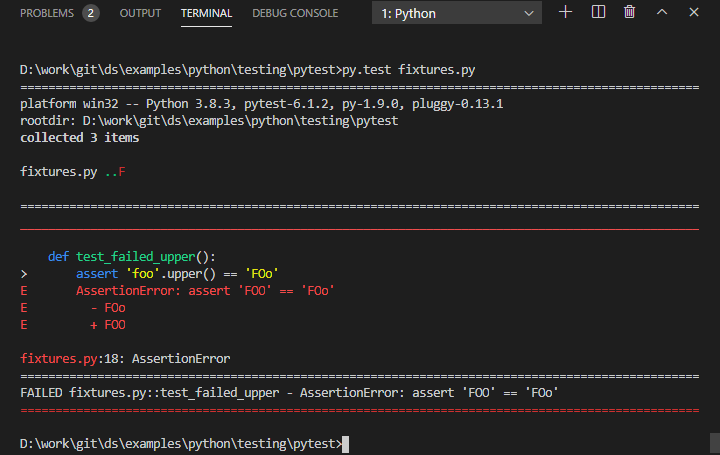
\includegraphics[scale=0.6]{images/pytest_run.png}
	\end{figure}
	См. также: https://habr.com/ru/post/269759/
\end{frame}

\end{document}